\documentclass[12pt]{article}

%----------Title & Cover-----------%
\title{Math 417: Abstract Algebra}
\author{Lanxiao Hermite Bai}
\date{\today}

%-----------Packeges---------------%
\usepackage{amsmath}
\usepackage{amssymb}
\usepackage{amsfonts}
\usepackage{tocloft}
\usepackage{float}
\usepackage{graphicx}
\usepackage[bookmarks=true]{hyperref}
\usepackage{fancyhdr}


%----------Definition & Theorem----%
\newtheorem{definition}{Definition}[subsection]
\newtheorem{theorem}{Theorem}[subsection]
\newtheorem{proposition}{Proposition}[subsection]
\newtheorem{lemma}{Lemma}[subsection]
\newtheorem{corollary}{Corollary}[subsection]


\pagestyle{fancy}
\fancyhead[L]{Math 417}
\fancyhead[C]{Note}
\fancyhead[R]{Lanxiao Bai}
%----------Document----------------%
\begin{document}
\maketitle
\newpage

\tableofcontents
\newpage

\section{Algebraic Themes}
    \subsection{Symmetry}
    \begin{definition}[Symmetry]
        A \textbf{symmetry} is an undetectable motion. An object is symmetric if it has symmetries.
    \end{definition}
    
\subsection{Multiplication Table}
\paragraph{Example of Multiplication Table}
Example of rectangle\\\\

\begin{table}[!hbp]
    \centering
    \begin{tabular}{c || c | c | c | c || c | c | c | c ||}
        
        & $e$ & $r$ & $r^2$ & $r^3$ & $a$ & $b$ & $c$ & $d$\\
        \hline
        \hline
           
           $e$ & $e$ & $r$ & $r^2$ & $r^3$ & $a$ & $b$ & $c$ & $d$\\
        \hline
           $r$ & $r$ & $r^2$ & $r^3$ & $e$ & $d$ & $c$ & $a$ & $b$\\
        \hline
           $r^2$ & $r^2$ & $r^3$ & $e$ & $r$ & $b$ & $a$ & $d$ & $c$\\
        \hline
            $r^3$ & $r^3$ & $e$ & $r$ & $r^2$ & $c$ & $d$ & $b$ & $a$\\
        \hline
        \hline
            $a$ & $a$ & $c$ & $b$ & $d$ & $e$ & $r^2$ & $r$ & $r^3$\\
        \hline
            $b$ & $b$ & $d$ & $a$ & $c$ & $r^2$ & $e$ & $r^3$ & $r$\\
        \hline
            $c$ & $c$ & $b$ & $d$ & $a$ & $r^3$ & $r$ & $e$ & $r^2$\\
        \hline
            $d$ & $d$ & $a$ & $c$ & $b$ & $r$ & $r^3$ & $r^2$ & $e$\\
        \hline\hline
    \end{tabular}
    \caption{Table of Multiplication for Rectangle}
\end{table}
    
\paragraph{Property of Symmetry}
\begin{enumerate}
    \item The product of symmetries is independent of how they are associated,
        \[
            s(tu) = (st)u
        \]

    \item  The \textit{nonmotion} $e$ compose with any other symmetry (in either order) is the second symmetry,
        \[
            eu = ue = u
        \]
    \item For each symmetry there is an inverse, such that the composition of the symmetry with its inverse (in either order) is the \textit{nonmotion} $e$,
        \[
            uu^{-1} = u^{-1}u = e
        \]
\end{enumerate}

\subsection{Symmetries and Matrices}
    \begin{definition}[Isometry]
        A transformation $\tau : R \rightarrow R$ is called an \textbf{isometry} if for all points $\mathbf {a, b} \in R$, we have $d(\tau(\mathbf a), \tau(\mathbf b)) =  d(\mathbf {a, b})$, where $d$ demotes the usual Euclidean distance function.
    \end{definition}

    \begin{proposition}
        Let $R$ denote a polygon or a polyhedron in three-dimensional space, locate with its centroid at the origin of coordinates. Then every symmetry if $R$ is the restriction to $R$ of a linear isometry of $\mathbb{R}^3$.
    \end{proposition}

\subsection{Permutations}
    \begin{definition}[Permutation]
        The symmetries of a configuration of identical objects are called \textbf{permutations}. There are $n!$ permutations for n objects. The set of all the permutations is denoted by $Sym(X) = S_n$.
    \end{definition}

                                                                                                                                                                                                                                                                    qq
\begin{enumerate}
    \item The multiplication of permutation is associative.
    \item There is an identity permutation $e$, which leaves each object in its original position.
    \item For each permutation $\sigma$, there is an inverse permutation $\sigma^{-1}$.
\end{enumerate}

    \begin{definition}[Cycle]
        A permutation that permutes several numbers cyclically and leave all other. numbers fixed is call a \textbf{cycle}.
    \end{definition}
    \begin{definition}[Disjoint]
        Two cycles are \textbf{disjoint} if each leaves the fixed numbers moved by each other.
    \end{definition}
    \begin{definition}[Order]
        A permutation $\pi$ is said to have \textbf{order} k if $k^{th}$ power of $\pi$ is the identity and no lower power of $\pi$ is the identity. \textbf{A k-cycle has order k.}
    \end{definition}
    \begin{theorem}
        Every permutation of a finite set can be written uniquely as a product of disjoint cycles.
    \end{theorem}

\subsection{Divisibility in the Integers}

    \begin{definition}[Integer]
        We denote the set of \textbf{integers} $\{0, \pm1, \pm2, \hdots\}$ by $\mathbb{Z}$.
    \end{definition}
    \begin{definition}[Natural Number]
     We denote the set of natural numbers $\{1,2,3,\hdots\}$ by $\mathbb{N}$.
    \end{definition}

    \begin{proposition} : Addition and Multiplication\\
        \begin{enumerate}
            \item Addition on $\mathbb{Z}$ is commutative and associative.
            \item 0 is an identity element for addition; $\forall a \in \mathbb{Z}, 0+a=a$.
            \item Every element a of $\mathbb{Z}$ has an additive inverse $-a$ that  $a + (-a) = 0$.
            \item Multiplication on $\mathbb{Z}$ is commutative and associative.
            \item 1 is is an identity element for multiplication; $\forall a \in \mathbb{Z}, 1a = a$.
            \item The distribute law holds; $a(b + c) = ab + ac$.
            \item $\mathbb{N}$ is closed under addition and multiplication.
            \item The product of non-zero integers is non-zero.
        \end{enumerate}
    \end{proposition}
    
    \begin{definition}[Divisibility]
        We say that an interger $a$ \textbf{divides} $b$, (or that $b$ is divisible by $a$), if there is an interger $q$ such that $aq = b$; we write $a|b$ for "$a$ divides $b$"
    \end{definition}

    \begin{proposition}
        Properties of Divisibility:\\\\
        Let a, b, c, u, and v denote integers.\\
        \begin{enumerate}
            \item If $uv = 1$, then $u = v = 1$ or $u = v = -1$.
            \item If $a|b$ and $b|a$, then $a = \pm b$.
            \item Divisibility is transitive; if $a|b$, $b|c$, then $a|c$.
            \item If $a|b$ and $a|c$, then $a | (sb+tc)$, where s and t are integers.
        \end{enumerate}

    \end{proposition}
    \begin{definition}[Prime]
        A natural number is \textbf{prime} if it is greater than 1 and not divisible by any natural number other than 1 and itself.
    \end{definition}
    \begin{proposition}
        Any natural number other than 1 can be written as a product of prime numbers.
    \end{proposition}
    \begin{theorem}
        There are infinitely many prime numbers.
    \end{theorem}
    \begin{proposition}
        Given integers $a$ and $b$, with $d \geq 1$, there exist unique intergers $q$ and $r$\footnote{The $q$ is called \textbf{quotient} and the $r$ is called \textbf{remainder}.} such $a = qd + r$ and $0 \leq r < d$.
    \end{proposition}
    \begin{definition}[Greatest Common Divisor]
        A natural number d is the greatest common divisor of nonzero integers m and n if\\
        \begin{enumerate}
            \item $d | m$ and $d | n$;
            \item whenever $x \in \mathbb{N}$ divides $m$ and $n$, then $x$ also divides $d$.
        \end{enumerate}
    \end{definition}

    \begin{proposition}
        For integers $m$ and $n$, let
        \begin{equation}
            I(m,n) = \{am+bn:a,b \in \mathbb{Z}\}.
        \end{equation}
        \begin{enumerate}
            \item For $x, y \in I(m,n)$, $x+y \in I(m, n)$ and $-x \in I(m,n)$.
            \item $\forall x \in \mathbb{Z}, xI(m, n) \subseteq I(m,n)$
            \item If $b \in \mathbb{Z}$ divides $m$ and $n$, then $b$ divides all elements of $I(m,n)$.
        \end{enumerate}
    \end{proposition}
    
    \begin{lemma}
        Let $m$ and $n$ be nonzero integers. If a natural number $d$ is a common divisor of $m$ and $n$ and an element of $I(m,n)$, then $d$ is the greatest common divisor of $m$ and $n$.
    \end{lemma}
    \begin{proposition}
        Let $m,n,n_1,...,n_k...,q_1,q_2,...q_k \in \mathbb{Z}$\\
        \begin{equation}
            m = q_1n+n_1
        \end{equation}
        
        \begin{equation}
            n = q_2n_1+n_2
        \end{equation}
        \centerline{...}
        \begin{equation}
            n_{k-2} = q_kn_{k-1}+n_k
        \end{equation}
        \centerline{...}
        \begin{equation}
            n_{r-1}=q_{r+1}n_r
        \end{equation}
        The natural number $n_r$ is the greatest common divisor of $m$ and $n$, and furthermore $n_r \in I(m, n)$.
    \end{proposition}
    \begin{corollary}
        Let $m$ and $n$ be nonzero integers, and write $d= g.c.d.(m,n)$
        \begin{enumerate}
            \item $d$ is the least element of $\mathbb{N} \cap I(m,n)$.
            \item $I(m,n) = \mathbb{Z}d$, the set of all integer multiples of $d$.
        \end{enumerate}
   \end{corollary}
    \begin{definition}[Relatively Prime]
        Nonzero integers $m$ and $n$ are \textbf{relatively prime} if $g.c.d.(m,n)$.
    \end{definition}
    \begin{corollary}
        Two nonzero integers $m$ and $n$ are relatively prime if and only if there exist integers $s$ and $t$ such that $1=sm+tn$.
    \end{corollary}
    \begin{corollary}
        Suppose that $a$ and $b$ are relatively prime natural numbers, that $x$ is an integer, and that both $a$ and $b$ divide $x$. Then $ab$ divides $x$.
    \end{corollary}
    
    \begin{proposition}
        If $p$ is a prime number and $a$ is any nonzero integer, then either $p$ divides $a$ or $p$ and $a$ are relatively prime.
    \end{proposition}
    
    \begin{proposition}
        Let $p$ be a prime number, and $a$ and $b$ nonzero integers. If $p|ab$, then $p|a$ or $p|b$. 
    \end{proposition}
    
    \begin{corollary}
        Suppose that a prime number $p|a_1a_2...a_r$, which for $r \in [1, r], a_n \neq 0$, then $p$ divides one of the factors.
    \end{corollary}
    
    \begin{theorem}
        The prime factorization of a natural number is unique.
    \end{theorem}
    \begin{definition}{Greatest common Divisor of Several Numbers}
        A natural nnumber $d$ is the greatest common divisor of nonzero integers $a_1, a_2, ..., a_n$, if
        \begin{enumerate}
            \item $d$ divides each $a_i$ and
            \item whenever $x \in \mathbb{N}$ divides each $a_i$, then $x$ also divides $d$.
        \end{enumerate}
    \end{definition}
    
    \begin{lemma}
        Given nonzero integers $a_1, a_2, ..., a_n(n \leq 2)$, there is a natural number $d$ and an n-by-n integer matrix $Q$ such that $Q$ is invertible, $Q^-1$ also has integer entries, and
        \begin{equation}
            (d, 0, ..., 0) = (a_1, a_2, ..., a_n)Q
        \end{equation}
    \end{lemma}

    \begin{proposition}
        The greatest common divisor of nonzero integers $a_1, a_2,...,a_n$ exists, and is an integer linear combination of $a_1, a_2, ..., a_n$.
    \end{proposition} 
    \begin{definition}[Relatively Prime]
        We say that nonzsro integers $a_1,...,a_n$ are \textbf{relatively prime} if their greatest common divisor is 1. We say that they are \textbf{pairwise relatively prime} if $a_i$ and $a_j$ are relatively prime whenever $i \neq j$.
    \end{definition}

\subsection{Modular Arithmetic}
    \begin{definition}[Congruence]
        Given integers $a$ and $b$, and a natural number $n$, we say that "$a$ is congruent to $b$ modulo $n$" and we write $a \equiv b \mod n$ if $n|(a-b)$.
    \end{definition}

    \begin{lemma}
        Properties of Mod
        \begin{enumerate}
            \item $\forall a \in \mathbb{Z}, a \equiv a\mod n$(Reflexive)
            \item $\forall a,b \in \mathbb{Z}$, if $a \equiv b \mod n$ if and only if $b \equiv a \mod n$.(Symmetric) 
            \item $\forall a,b,c \in \mathbb{Z}$, if $a \equiv b \mod n$ and $b \equiv c \mod n$, then $a \equiv v \mod n$.(Transitive)
        \end{enumerate}
    \end{lemma}
    
    \begin{lemma}
        For $a, b \in \mathbb{Z}$, the following are equivalent:
        \begin{itemize}
            \item $a \equiv b \mod n$.
            \item $[a] = [b]$.\footnote{The set Œa  is called the residue class or congruence class of a modulo n.}
            \item $rem_n(a) = rem_n(b)$.\footnote{Denote by $rem_n(a)$ the unique number $r$ such that $0 \leq r < n$ and $a-r$ is divisible by $n$.}
            \item $[a]\cap[b] \neq \varnothing$
        \end{itemize}
    \end{lemma}

    \begin{corollary}
        There exist exactly $n$ distinct residue classes modulo $n$, namely $[0],[1],...[n-1]$. These classes are mutually disjoint.
    \end{corollary}
    \begin{lemma}
        Let $a, a',b ,b'$ be integers with $a \equiv a' \mod n$ and $b \equiv b\ \mod n$. Then $a+b \equiv a'+b' \mod n$ and $ab \equiv a'b' \mod n$.
    \end{lemma}

    \begin{proposition}
        Properties of Modulo Congruence:\\
        \begin{enumerate}
            \item Addition on $\mathbb{Z}_n$ is commutative and associative, $\forall [a], [b], [c] \in \mathbb{Z}_n$
                \begin{equation}
                   [a]+[b]=[b]+[a]
                \end{equation}
                and,
                \begin{equation}
                    [a]+[b]+[c] = [a]+([b]+[c])
                \end{equation}
            \item [0] is an identity element for addition, $\forall [a] \in \mathbb{Z}_n$,
                \begin{equation}
                    [0]+[a]=[a]
                \end{equation}
            \item Every element $[a]$ of $\mathbb{Z}_n$ has an additive inverse $[-a]$, that
                \begin{equation}
                    [a] + [-a] = [0]
                \end{equation}

            \item Muktiplication on $\mathbb{Z}_n$ is commutative and associative; $\forall [a], [b], [c] \in \mathbb{Z}_n$,
                \begin{equation}
                    [a][b] = [b][a]
                \end{equation}
                ,and
                \begin{equation}
                    [a][b][c] = [a]([b][c])
                \end{equation}
            \item $[1]$ is an identity for multiplication; $\forall [a] \in \mathbb{Z}_n$,
                \begin{equation}
                    [1][a] = [a][1]
                \end{equation}
            \item The distributive law hold; $\forall [a], [b], [z] \in \mathbb{Z}_n$,
                \begin{equation}
                    [a]([b]+[c]) = [a][b] + [a][c]
                \end{equation}
        \end{enumerate}
    \end{proposition}

    \begin{proposition}[Chinese Reminder Theorem]
        Suppose $a$ and $b$ are relatively prime natural numbers, and $\alpha$ and $beta$ are integers. There exists an integer $x$ such that $x \equiv \alpha \mod a$ and $x \equiv \beta \mod b$. Moreover, $x$ is unique up to congruence modulo $ab$.
    \end{proposition}

\subsection{Polynomials}
    \paragraph{Denotation} Denote set of rational numbers by $\mathbb{Q}$, and denote set of real numbers by $\mathbb{R}$ and denote set of complex numbers by $\mathbb{C}$.
    \paragraph{Addition and Multiplication}
    \begin{equation}
        (\sum_j a_jx^j)+(\sum_j b_jx^j) = \sum_j(a_j+b_j)x^j
    \end{equation}
    and,
    \begin{equation}
        (\sum_i a_ix^i)(\sum_j b_jx^j) = \sum_i\sum_j(a_ib_j)x^{i+j}
    \end{equation}
    \begin{equation}
        =\sum_k(\sum_{i,j:i+j=k}a_ib_j)x^k = \sum_k(\sum_i a_ib_{k-i})x^k
    \end{equation}

    \begin{proposition}
        Basic Properties:\\
        \begin{enumerate}
            \item Addition in $K[x]$ is commutative and associative; $f+g=g+f$ and $\forall f,g,h \in K[x], f+g+h=f+(g+h)$.
            \item 0 is an identity element for addition; $0+f = f$.
            \item Every element $f$ of $K[x]$ has an additive inverse $-f$; $f + (-f) = 0$.
            \item Multiplication in $K[x]$  is commutative and associative; that is, for all $f, g, h \in K[x]$, $fg=gf$, and $f(gh)=(fg)h$.
            \item 1 is an identity for multiplication; $\forall f \in K[x], 1f=f$.
            \item The distributed law holds; $\forall f, g, h \in K[x], f(g+h)=fg+fh$.
        \end{enumerate}

    \end{proposition}
    \begin{definition}[Degree]
        The \textbf{degree} of a polynomial $\sum_k a_kx^k$ is the largest $k$ that $a_k \neq 0$. If $p=\sum_j a_jx^j$ is a nonzero polynomial of degree k, denoted $deg(p)$, the \textbf{leading coefficient} of $p$ is $a_k$ and leading term of $p$ is $a_kx^k$. A polynomial is said to be \textbf{monic} if its leading coefficient is 1.   
    \end{definition}
    \begin{proposition}
        Let $f,g \in K[x]$.
        \begin{enumerate}
            \item $deg(fg)=deg(f)+deg(g)$; in particular, if $f$ and $g$ are both nonzero, then $fg \neq 0$.
            \item $deg(f+g) \leq \max\{deg(f), deg(g)\}$
        \end{enumerate}
    \end{proposition}
    
    \begin{proposition}
        Let $f, g, h, u, v$ denote polymonials like in $K[x]$.
        \begin{enumerate}
            \item If $uv = 1$, then $u, v \in K$.
            \item If $f|g and g|f$, then there is a $k \in K$ such that $g = kf$.
            \item Divisibility is transitive
            \item If $f|g$ and $f|h$, then $\forall s, t \in K[x], f|(sg+th)$.
        \end{enumerate}
    \end{proposition}

    \begin{definition}[Irreducible]
        We say that a polymonial in $K[x]$ is \textbf{irreducible} if its degree is positive and it cannot be written as a product of two polynomials each of strictly smaller (positive)degree.
    \end{definition}
    \begin{proposition}
        Any polynomial in $K[x]$ of positive degree can be written as a product of irrecucible polynomials.
    \end{proposition}
    \begin{proposition}
        $K[x]$ contains infinitely many irreducible polynomials.
    \end{proposition}
    \begin{lemma}
        Let $p$ and $d$ be elements of $K[x]$, with $deg(p) \geq deg(d) \geq 0$. Then there is a monomial $m = bx^k \in K[x]$ and a polynomial $p' \in K[x]$ such that $p = md + p'$, and $deg(p') < deg(p)$.
    \end{lemma}

    \begin{proposition}
        Let $p, d \in K[x]$, with $deg(d) \geq 0$. Then there exist polynommials $q$ and $r$ in $K[x]$ such that $p = dq+r$ and $deg(r) < deg(d)$.
    \end{proposition}
    \begin{definition}[Great Common Divisor of Polynomials]
        A polynomial $f\in K[x]$ is a greatest common divisor of nonzero polynomials $p,q \in K[x]$ if
        \begin{enumerate}
            \item $f|p$ and $f|q$ in $K[x]$ and
            \item whenever $g \in K[x]$ divides $p$ and $q$, then $g$ also divides $f$.
        \end{enumerate}

    \end{definition}

    \begin{proposition}
        For polynomials $f,g \in K[x]$, let
        \begin{equation}
            I(f,g) = {af+bg:a,b \in K[x]}
        \end{equation}
        \begin{enumerate}
            \item $\forall p,q \in I(f,g), p+q\in I(f,g)$ and $-p\in I(f,g)$
            \item $\forall p \in K[x]$, $pI(f,g) \subseteq I(f,g)$.
            \item If $p \in K[x]$ divides $f$ and $g$, then $p$ divides all elements in $I(f,g)$.
        \end{enumerate}

    \end{proposition}
    
    \begin{theorem}
        ANy two nonzero polynomials $f,g \in K[x]$ have a greatest common divisor $\in I(f,g)$.
    \end{theorem}
    \begin{definition}[Relatively Prime]
        Two polynomials $f,g \in K[x]$ are \textbf{relatively prime} if $g.c.d.(f,g) = 1$.
    \end{definition}
    \begin{proposition}
        Two polynomials $f,g \in K[x]$ are relatively prime if and only if $1 \in I(f,g)$.
    \end{proposition}
    \begin{proposition}
        Properties of irreducible polynomial\\
        \begin{enumerate}
            \item Let $p$ be an irreducible polynomial in $K[x]$ and $f,g \in K[x]$ nonzero polynomials. If $p | fg$, then $p|f$ or $p|g$.
            \item Suppose that irreducible polynomial $p \in K[x]$ divides a product $f_1f_2...f_s$ of nonzero polynomials. Then $p$ divides one of the factors.
        \end{enumerate}
    \end{proposition}

    \begin{theorem}
        The factorization of a polynomial in $K[x]$ into irreducible factors is essentially unique.
    \end{theorem}

    \begin{proposition}
        Let $p \in K[x]$ and $a \in K$. Then there is a polynomial $q$ such that $p(x) = q(x)(x-a) + p(a)$. Consequently, $p(a) = 0$ if and only if $(x-a)|p$.
    \end{proposition}
    
    \begin{definition}[Root]
        An element $\alpha \in K$ is a \textbf{root} of a polynomial $p \in K[x]$ if $p(\alpha)=0$. The \textbf{multiplication of the root $\alpha$} is $k$ if $x-\alpha$ appears exactly $k$ times in the irreducible pfactorization of $p$.
    \end{definition}
    
    \begin{corollary}
        A polynomial $p \in K[x]$ of degree $n$ has at most $n$ roots in $K$, counting with multiplicities.
    \end{corollary}

\subsection{Counting}
    \begin{proposition}
        A set with $n$ elements has $2^n$ subsets.
    \end{proposition}
    	\paragraph{Proof:} \[N = \sum_{i = 0}^n \binom{n}{i} = 2^n\]
    
    \begin{proposition}
        Let $n$ be a natural number and let $k$ be an integer in $[0,n]$. Let $\left(\begin{array}{c} n\\k\\\end{array}\right)$ denote the number of the number of k-element subsets of a set with $n$ elements. Then
        \begin{equation}
            \left(\begin{array}{c} n\\k\\\end{array}\right) = \frac{n!}{k!(n-k)!}
        \end{equation}
        If $k < 0$ or $k > n$,
        \begin{equation}
            \left(\begin{array}{c} n\\k\\\end{array}\right) = 0
        \end{equation}
        and,
        \begin{equation}
            \left(\begin{array}{c} 0\\0\\\end{array}\right) = 1
        \end{equation}
        \begin{equation}
            \left(\begin{array}{c} 0\\k\\\end{array}\right) = 0
        \end{equation}
if $k \neq 0$

    \end{proposition}
    \begin{lemma}
        Let $n$ be a natural number and $k \in \mathbb{Z}$.
        \begin{enumerate}
            \item $\left(\begin{array}{c} n\\k\\\end{array}\right)$ is a nonnegative integer.
            \item $\left(\begin{array}{c} n\\k\\\end{array}\right) = \left(\begin{array}{c} n\\n-k\\\end{array}\right)$.
            \item $\left(\begin{array}{c} n\\k\\\end{array}\right) = \left(\begin{array}{c} n-1\\k\\\end{array}\right) + \left(\begin{array}{c} n-1\\k-1\\\end{array}\right)$ 
        \end{enumerate}

    \end{lemma}
    \begin{proposition}[Binomial Theorem]
        Let $x$ and $y$ be numbers. For $n \geq 0$, we have
        \begin{equation}
            (x+y)^n = \sum^n_{k=0}\left(\begin{array}{c} n\\k\\\end{array}\right)x^ky^{n-k}
        \end{equation}

    \end{proposition}
    \begin{corollary}
            Basic Properties:
        \begin{enumerate}
            \item
                \begin{equation} 
                2^n = \sum^n_{k=0}\left(\begin{array}{c} n\\k\\\end{array}\right)
                \end{equation}
            \item
                \begin{equation} 
                0 = \sum^n_{k=0}(-1)^k\left(\begin{array}{c} n\\k\\\end{array}\right)
                \end{equation}
            \item
                \begin{equation} 
                2^{n-1} = \sum^n_{k=0, k\ odd}\left(\begin{array}{c} n\\k\end{array}\right) = \sum^n_{k=0, k\ even}\left(\begin{array}{c} n\\k\\\end{array}\right)
                \end{equation}
        \end{enumerate}

    \end{corollary}
    \begin{lemma}
        Let $p$ be a prime number.
        \begin{enumerate}
            \item If $0 < k < p$, then $\left(\begin{array}{c} p\\k\\\end{array}\right)$ is divisible by $p$.
            \item $\forall a, b \in \mathbb{Z}, (a+b)^p \equiv a^p + b^p \mod p$.
        \end{enumerate}

    \end{lemma}
    \begin{proposition}
        .\\
        \begin{enumerate}
            \item Let $n \geq 2$ be a natural number. An element $[a] \in \mathbb{Z}_n$ has a multiplicative inverse if and only if $a$ is relatively prime to $n$.
            \item If $p$ is a prime, then every nonzero element of $\mathbb{Z}_p$ is invertible.
        \end{enumerate}

    \end{proposition}
    \begin{proposition}[Fermat's Little Theorem]
        Let $p$ be a prime number.
        \begin{enumerate}
            \item $\forall a \in \mathbb{Z}, a^p \equiv a \mod p$.
            \item If $p \nmid a, a^{p-1} \equiv 1 \mod p$.
        \end{enumerate}

    \end{proposition}
    \begin{definition}[Characteristic Function of X]
        Let $U$ be any set, for a subset $X \subseteq U$, the \textbf{characteristic function} of X is the function $\textbf{1}_X:U\rightarrow {0,1}$ defined by 
        \begin{equation}
            \textbf{1}_X(u) = \left\{ \begin{array}{ll}1 & \mathrm{if\ }u \in X\\ 0 & \mathrm{if\ }u \notin X \end{array}\right.
        \end{equation}
    \end{definition}
    \paragraph{Denotation}
        Denote The relative copmplement of a subset $X \subseteq U$ by $X'$.
    \begin{proposition}
        Let $A_1, A_2, ..., A_n \subseteq U$, then
        \begin{enumerate}
            \item
            \begin{equation} 
                \textbf{1}_{A'_1 \cap A'_2 \cap ...\cap A'_n} = 1-\sum_i \textbf{1}_{A_i} + \sum_{i<j}\textbf{1}_{A_i \cap A_j} - \sum_{i < j < k}\textbf{1}_{A_i \cap A_j \cap A_k} + ... + (-1)^n\textbf{1}_{A_1\cap ...\cap A_n}
            \end{equation}
            \item
            \begin{equation}
                \textbf{1}_{A_1 \cup A_2 \cup ...\cup A_n} = \sum_i \textbf{1}_{A_i} - \sum_{i<j}\textbf{1}_{A_i \cap A_j} + \sum_{i < j < k}\textbf{1}_{A_i \cap A_j \cap A_k} - ... + (-1)^n\textbf{1}_{A_1\cap ...\cap A_n}
            \end{equation}

        \end{enumerate}

    \end{proposition}

    \begin{corollary}
        Suppose that $U$ is a finite set and that $A_1, A-2, ..., A_n$ are subsets of $U$. Then
        \begin{enumerate}
            \item
                \begin{multline}
                    |A'_1\cap A'_2\cap ...\cap A'_n| = |U|-\sum_i|A_i|+\sum_{i<j}|A_i \cap A_j| - \sum_{i < j < k}|A_i \cap A_j \cap A_k| + ... +(-1)^n |A_1 \cap ... A_n|
                \end{multline}
            \item
                \begin{multline}
                    |A_1\cup A_2\cup ... \cup A_n| = \sum_i |A_i| - \sum_{i<j}|A_i \cap A_j| + \sum_{i < j < k}|A_i \cap A_j \cap A_k| - ... +(-1)^n |A_1 \cap ... A_n|
                \end{multline}

        \end{enumerate}

    \end{corollary}
    \begin{definition}[Cardinality]
        For each natural number n, $\varphi(n)$ is defined to be the cardinality of the set of natural numbers $k < n$ such that $k$ is relatively prime to $n$. 
    \end{definition}
    \begin{lemma}
        Let $k, n \in \mathbb{N}$, with $k|n$. The number of natural numbers $j \leq n$ such that $k|j$ is $n/k$.
    \end{lemma}
    \begin{corollary}
        If $p$ is a prime, then $\forall k \geq 1$, $\varphi(p^k) = p^{k-1}(p-1)$.
    \end{corollary}
    \begin{proposition}
        Let $n$ be a natural number with prime factorization $n=p^{k_1}_1...p^{k_s}_s$. Then,
        \begin{enumerate}
            \item 
                \begin{equation}
                    \varphi(n)=n\prod_{i=1}^s (1-\frac{1}{p_i})
                \end{equation}
            \item
                \begin{equation}
                    \varphi(n)=\prod_{i=1}^s \varphi(p^{k_i}_i)
                \end{equation}
        \end{enumerate}
    \end{proposition}

    \begin{corollary}
        If $m$, $n$ are relatively prime, then $\varphi(mn) = \varphi(m)\varphi(n)$.
    \end{corollary}
    
    \begin{theorem}[Euler's Theorem]
        Fix a natural number $n$. If $a \in \mathbb{Z}$ is relatively prime to n, then
        \begin{equation}
            a^{\varphi(n)} \equiv 1 \mod n.
        \end{equation}

    \end{theorem}

\subsection{Groups}

\paragraph{Operation} An \textit{operation} or a \textit{product} on a set $G$ is a function from $G \times G$ to $G$.
\begin{definition}[Group]
    A \textbf{group} is a nonempty set $G$ with a product, denoted by juxtaposition, satisfying:
    \begin{enumerate}
        \item Associativity: The product is associative: $\forall a,b,c \in G, (ab)c = a(bc)$.
        \item Identity element: There is an identity element $e \in G, a \in G, ea = ae = a$.
        \item Inserse element: For each $a \in G$, there is $a^{-1} \in G, aa^{-1} = a^{-1}a = e$.
        \item Closure: For any $a, b \in G$, $ab \in G$.
    \end{enumerate}

\end{definition}
\paragraph{Isomorphic} Groups $G$ and $H$ is said to be \textbf{isomorphic} if there is a biject map $\varphi: H \rightarrow G$ between them that makes the multiplication table match up, namely, $\forall g_1,g_2 \in G$, $\varphi(g_1g_2) = \varphi(g_1)\varphi(g_2)$.\footnote{Denote as $H \cong G$}

\paragraph{Subgroup} If $G \subseteq H$, $G$ is said to be the \textbf{subgroup} of H.

\paragraph{Homomorphism} A map $f: H\rightarrow G$ is said to be \textbf{homomorphism} if $f$ take products to products, identity to identity, and inverses to inverses, $f(a\cdot b)=f(a)\cdot f(b)$.

\begin{lemma}
    The set $\Phi(n)$ of elements in $\mathbb{Z}_n$ prossessing a multiplicative inverse forms a group (of cardinality $\varphi(n)$) under multiplication, with identity element $[1]$.
\end{lemma}

\subsection{Rings and Fields}

\begin{definition}
    A \textbf{ring} is a nonempty set $R$ with two operations: addition, donated by $+$ and multiplication, donated by juxtaposition that satisfy:
    \begin{enumerate}
        \item Under addition, $R$ is an \textbf{Abelian group}.\footnote{Abelian group is a group that holds communitative law; For $a, b \in R$, $ab = ba$.}
        \item Multiplication is associative.
        \item Multiplication distributes over addition:$\forall a,b,c\in R, a(b+c) = ab+ac$ and $(b+c)a = ba+ca$ \footnote{If multiplication is commutative, the ring is called a \textbf{commutative ring}.}

    \end{enumerate}
   \end{definition}

\paragraph{Subring} If $G \subseteq H$, $G$ is said to be the \textbf{subring} of H.

\begin{proposition}[Chinese Remainder Theorem]
    Let a and b be relatively prime natural numbers, each then there is an isomorphism of rings
    \begin{equation}
        \mathbb{Z}_{ab} \cong \mathbb{Z}_a \oplus \mathbb{Z}_b
    \end{equation}
    defined by $[x]_{ab} \mapsto ([x]_a, [x]_b)$.
\end{proposition}

\begin{definition}
    A \textbf{field} is a commutative ring with multiplicative identity element $1 \neq 0$ which every nonzero element is a unit.\footnote{Unit in ring means the multiplicationally invertible elements}
\end{definition}

\subsection{An application to cryptology}

\begin{lemma}
    For all integers a and h, if $h \equiv 1 \mod m$, then $a^h \equiv a \mod n$.
\end{lemma}
\begin{lemma}
    $\forall a \in \mathbb{Z}$, if $b \equiv a^r \mod n$, then $b^s \equiv a \mod n$.
\end{lemma}

\section{Basic Theory of Groups}
    \subsection{First Results}
    \begin{proposition}[Uniqueness of the identity]
        Let G be a group and suppose e and $e'$ are both identity elements in G, then $e = e'$.
    \end{proposition}
    \begin{proposition}[Uniqueness of the inverse]
        Let G be a group and $h, g \in G$. If $hg = e$, then $h = g^{-1}$, and if $gh = e$, then $h=g^{-1}$.
    \end{proposition}
    
    \begin{corollary}
        Let $g \in G$, then $g = (g^{-1})^{-1}$.
    \end{corollary}

    \begin{proposition}
        Let G be a group and $a, b \in G$. Then $(ab)^{-1} = b^{-1}a^{-1}$. 
    \end{proposition}

    \begin{proposition}
        Let G be a group and $a \in G$, The map $L_a:G\rightarrow G$ defined by $L_a(x)=ax$ is a bijectiion. Similarly $R_a(x)=xa$ is a bijection.
    \end{proposition}
    
    \begin{corollary}
        Let G be a group and $a, b \in G$. The equation $ax=b$ has a unique solution x in G, and likewise the equation $xa = b$ has a unique solution in G.
    \end{corollary}
    
    \begin{corollary}[Cancellation]
        Suppose $a, x, y \in G$. If $ax = ay$, then $x = y$. If $xa = ya$, then $x = y$.
    \end{corollary}

    \begin{corollary}
        If G is a finite group, each row and each column of the multiplication table of G contains each element of G exactly once.
    \end{corollary}
    
    \begin{definition}[Order]
        The \textbf{order} of a group is its size or cardinality, denote by $|G|$.
    \end{definition}

    \begin{definition}[Isomorphic]
        We say that two groups G and H are \textbf{isomorphic} if there is a bijection $\varphi:G\rightarrow H$ such that for all $g_1, g_2 \in G$, $\varphi(g_1g_2) = \varphi(g_1)\varphi(g_2)$. The map is called an \textbf{isomorphism}.
    \end{definition}
    
    \begin{definition}[Abelian]
        A A group G is called \textbf{abelian (or commutative)} if for all elements $a, b \in G$, the products in the two orders are equal: $ab = ba$.
    \end{definition}
    
    \begin{proposition}
        Properties of isomorphism:
        \begin{enumerate}
            \item Up to isomorphism, $\mathbb{Z}_1$ is the unique group of order 1.
            \item Up to isomorphism, $\mathbb{Z}_2$ is the unique group of order 2.
            \item Up to isomorphism, $\mathbb{Z}_3$ is the unique group of order 3.
            \item Up to isomorphism, there are exactly two groups of order 4, namely $\mathbb{Z}_4$, and the group of rotational symmetries of the rectangular card.
            \item Up to isomorphism, $\mathbb{Z}_5$ is the unique group of order 5.
            \item All groups of order no more than 5 are abelian.
            \item There are at least two nonisomorphic groups of order 6, one
abelian and one nonabelian.
         \end{enumerate}
    \end{proposition}
    
    \begin{proposition}[General associative law]
        Let M be a set with an associative operation, $M \times M \rightarrow M$, denoted by juxtaposition. FOr every $n \geq 1$, there is a unique product $M^n \rightarrow M$,
        \[(a_1, a_2, ..., a_n) \mapsto a_1a_2...a_n,\]
        such that
        \begin{enumerate}
            \item The product of one element is that element $(a) = a$.
            \item The product of two elements agrees with the given operation $(ab) = ab$
            \item $a_1a_2...a_n = (a_1 ... a_k)(a_{k+1}...a_n).$
        \end{enumerate}

    \end{proposition}
\subsection{Subgroup and Cyclic Groups}
    \begin{definition}[Subgroup]
        A nonempty subset H of a group G is called a subgroup if H is itself a group with the group operation inherited from G. We write $H \leq G$ to indicate that H is a subgroup of G.
    \end{definition}
    
    \begin{proposition}
        Let G be a group and let $H_1, H_2, \cdots, H_n$ be subgroups of G. Then $H_1\cap H_2\cap \cdots\cap H_n$ is a subgroup of G. More generally, if $\{H_{\alpha}\}$ is any collection of subgroups, then $\cap_{\alpha}H_{\alpha}$ is a subgroup.
    \end{proposition}
    \begin{proposition}
        Let a be an element of a group G. The subgroup $\langle a\rangle$ generated by a is $\{a^k : k\in \mathbb{Z}\}$\footnote{For any group G and any subset $S \subseteq G$, there is a smallest subgroup of G that contains S, which is called the subgroup generated by S.}
    \end{proposition}
    \begin{definition}[Cyclic Group]
        Let a be an element of a group G. The set $\langle a \rangle = \{a^k : k \in \mathbb{Z}\}$ of powers of a is called the cyclic subgroup generated by a. If there is an element $a \in G$ such that $\langle a \rangle = G$, we say that G is a cyclic group. We say that a is a generator of the cyclic group.
    \end{definition}
    \begin{definition}[Order]
        The order of the cyclic subgroup generated by a is called the order of a. We denote the order of a by $o(a)$.
    \end{definition}
    
    \begin{proposition}
    	If $G$ is a cyclic group and $g \in G$, $o(g) = |G|/g.c.d(g, |G|)$
    \end{proposition}
    	\paragraph{Proof}
    	In $\mathbb{Z}_n, g \in \mathbb{Z}_n$, $kg \equiv 0 \mod n \Leftrightarrow kg = ln = \mathrm{lcm}(g, n)$.
    	
    	Since $g.c.d(g, n)\cdot l.c.m(g, n) = gn$, $o(g) = n = |G|/g.c.d(g, |G|)$.$\blacksquare$

    \begin{proposition}
       If the order of a is finite, then it is the least positive integer n such that $a^n = e$. Furthermore, $\langle a \rangle = \{a^k: 0 \leq k < o(a)\}$.
    \end{proposition}
    \begin{proposition}
        Let H be a subgroup of $\mathbb{Z}$. Then either $H = {0}$, or there is a unique $d \in \mathbb{N}$ such that $H = \langle d \rangle = d\mathbb{Z}$.
    \end{proposition}
    \begin{proposition}
        If $d \in \mathbb{N}$, then $d\mathbb{Z} \cong \mathbb{Z}$.
    \end{proposition}
    \begin{proposition}
        If $a, b \in \mathbb{N}$, then $a\mathbb{Z} \subseteq b \mathbb{Z}$ if and only if $b | a$.
    \end{proposition}
    \begin{corollary}
        Every subgroup of $\mathbb{Z}$ other than ${0}$ is isomorphic to $\mathbb{Z}$.
    \end{corollary}
    \begin{lemma}
        Let $n \geq 2$ and let d be a positive divisor of n. The cyclic subgroup $\langle [d] \rangle$ generated by $[d]$ in $\mathbb{Z}_n$ has cardinality $|\langle [d] \rangle | = n/d$
    \end{lemma}
    \begin{proposition}
        Let H be a subgroup of $\mathbb{Z}_n$.
        \begin{enumerate}
            \item Either $H = {[0]}$, or there is a $d > 0$ such that $H = \langle [d] \rangle$.
            \item If d is the smallest of positive intefers s such that $H = \langle [s] \rangle$, then $d|H| = n$.
        \end{enumerate}

    \end{proposition}
    \begin{corollary}
        Fix a natural number $n \geq 2$.
        \begin{enumerate}
            \item Any subgroup of $\mathbb{Z}_n$ is cyclic.
            \item Any subgroup of $\mathbb{Z}_n$ has cardinality dividing n.
        \end{enumerate}

    \end{corollary}
    \begin{corollary}
        Fix a natural number $n \geq 2$.
        \begin{enumerate}
            \item For any positive divisor q of n, there is a unique subgroup of $\mathbb{Z}_n$ of cardinality q, namely $\langle [n/q] \rangle$.
            \item     For any two subgroups H and H' of $\mathbb{Z}_n$, we have $H \subseteq H' \Leftrightarrow$ $|H|$ divides $|H'|$.
        \end{enumerate}
    \end{corollary}

    \begin{proposition}
            Every subgroup of a cyclic group is cyclic.
    \end{proposition}
    \begin{proposition}
        Let a be an element of finite order n in a group. Then $\langle a^k \rangle = \langle a \rangle$, if and only if k is relatively prime to n. The number of generators of $\langle a \rangle$ is $\varphi(n)$.
    \end{proposition}
    \begin{proposition}
        Let a be an element of finite order n in a group. For each positive integer q dividing n, $\langle a \rangle$ has a unique subgroup of order q.
    \end{proposition}
    \begin{proposition}
        Let a be an element of finite order n in a group. For each nonzero integer s, as has order $n=g.c.d.(n, s)$.
    \end{proposition}
\subsection{The Dihedral Groups}
    \begin{definition}[Dihedral Group]
        Group consists of n rotational symmetries and n reflection symmetries is a \textbf{dihedral group}, denoted by $D_n$.
    \end{definition}
	\begin{proposition}
		$D_n = <r, a | r^n = e, a^2 = e, ra = ar^{-1}>$ 
	\end{proposition}
    \paragraph{Properties:}
        \begin{enumerate}
            \item $jr_t = r_{-t}j$ and $j_t = r_{2t}j = jr_{-2t}$.
            \item All products in D can be computed using these relations.
            \item The symmetry group D of the disk consists of the rotations $r_t$ for $t\in\mathbb{R}$ and the flips $j_t = r_{2t}j$. Writing $N = {r_t : t\in\mathbb{R}}$, we have $D = N \cup Nj$.
            \item The subgroup N of D satisfies $aNa^{-1} = N$ for all $a \in D$.
        \end{enumerate}

\subsection{Homomorphisms and Isomorphisms}
    \begin{definition}[Homomorphism]
        A map between groups $\varphi: G \rightarrow H$ is called a \textbf{homomorphism} if it preserves group multiplication, $\varphi(g_1g_2) = \varphi(g_1)\varphi(g_2)$ for all $g_1, g_2 \in G$. And An endomorphism of G is a homomorphism $\varphi: G \rightarrow G$.
    \end{definition}
    \begin{proposition}
    	If  $\varphi: G \rightarrow H$ and $\psi: H \rightarrow K$ are both group hom, then $\varphi \circ \psi: H \rightarrow K$ is a group hom.
    \end{proposition}
    \begin{proposition}
    	If $\varphi: G \rightarrow H$ be a homomorphism of groups.
    		\begin{itemize}
    			\item $\varphi(e_G) = e_H$
    			\item $\forall g \in G, \varphi(g^{-1}) = (\varphi(g))^{-1}$
    		\end{itemize}
    \end{proposition}
    \begin{proposition}
        Let $\varphi: G \rightarrow H$ be a homomorphism of groups.
        \begin{enumerate}
            \item For each subgroup $A \subseteq G$, $\varphi(A) \subseteq H$. (Image of A)
            \item For each subgroup $B \subseteq G$,
            \[\varphi^{-1}(B) = {g \in G: \varphi(g)\in B}\]
            is a subgroup of G. (Inverse image of B)
        \end{enumerate}
    \end{proposition}
    \subsubsection{The Kernel of a Homomorphism}
    \begin{definition}[Normal]
        A subgroup N of a group G is said to be \textbf{normal} if $\forall g \in G$, $gNg^{-1}=N$. Here $gNg^{-1}$ means ${gng^{-1} : n \in N}$.\footnote{$gng^{-1}$ is called conjugate if $n$ by $g$}\footnote{Denote as $N \trianglelefteq G$}
    \end{definition}
    \begin{corollary}
    	\[A_n \trianglelefteq S_n\]
    \end{corollary}
    \begin{proposition}
        If a subgroup N of a group G is its \textbf{normal subgroup}, then $\forall g \in G$, $gN = Ng$.
    \end{proposition}
    
    \begin{proposition}
    	Any subgroup of Abelian group is normal.
    \end{proposition}

    \begin{definition}[Kernel]
        Let $\varphi: G \rightarrow H$ be a homomorphism of groups. The \textbf{kernel} of the homomorphism $\varphi$, denoted $ker(\varphi)$, is $\varphi^-1(e_H) = \{g \in G: \varphi(g) = e_H\}$.\footnote{$e_H$ is the identity of group H.}
    \end{definition}
    \paragraph{e.g.1}
    $\varphi: \mathbb{Z} \rightarrow \mathbb{Z}_2$, \[\mathrm{ker}(\varphi) = \{a \in \mathbb{Z} | [a] = [0]\}\]
    \paragraph{e.g.2}
    $\mathrm{det}: GL(\alpha, \mathbb{R}) \rightarrow \mathbb{R}^*$
    \[\mathrm{ker}(\mathrm{det}) = \mathrm{SL}(\alpha, \mathbb{R})\]
    \begin{proposition}
        A homomorphism $\varphi: G \rightarrow H$ is injective if and only if $ker(\varphi) = {e_G}$.
    \end{proposition}
    \begin{proposition}
        Let $\varphi: G \rightarrow H$ be a homomorphism of groups. Then $ker(\varphi)$ is a normal subgroup of G.
    \end{proposition}


    \subsubsection{Parity of Permutations}
        \begin{definition}[Sign, Parity]
            The homomorphism $\epsilon$ is called the \textbf{sign} (or \textbf{parity}) homomorphism. A permutation $\pi$ is said to be even if $\epsilon(\pi) = 1$, that is, if $\pi$ is in the kernel of the sign homomorphism. Otherwise, $\pi$ is said to be odd. The subgroup of even permutations (that is, the kernel of $\epsilon$) is generally denoted $A_n$. This subgroup is also referred to as the alternating group.\footnote{$(a_1a_2\cdots a_{l-1}a_{l}) = \prod_{i = 0}^{l - 2}(a_1a_{l - i})$}
        \end{definition}
        \begin{proposition}
            A permutation $\pi$ is even if and only if $\pi$ can be written as a product of an even number of 2-cycles.
        \end{proposition}

        \begin{corollary}
            The set of odd permutations in $S_n$ is $(12)A_n$, where $A_n$ denotes the subgroup of even permutations.
        \end{corollary}
    
        \begin{corollary}
            A k-cycle is even if k is odd and odd if k is even.
        \end{corollary}
    
    \subsection{Cosets and Lagrange’s Theorem}
    
    \begin{definition}[Coset]
        Let H be subgroup of a group G. A subset of the form gH, where $g \in G$, is called a left coset of H in G. A subset of the form Hg, where $g \in G$,is called a right coset of H in G.
    \end{definition}

    \subsubsection{Properties of Cosets}
    \begin{proposition}
        Let H be a subgroup of a group G, and let a and b be elements of G. The following conditions are equivalent:
        \begin{enumerate}
            \item $a\in bH$.
            \item $b\in aH$
            \item $aH = bH$.
            \item $b^{-1}a \in H$.
            \item $a^{-1}b \in H$.
        \end{enumerate}

    \end{proposition}
    
    \begin{proposition}
        Let H be a subgroup of a group G.
        \begin{enumerate}
            \item Let a and b be elements of G. Either $aH = bH$ or $aH \cap bH = \emptyset$.
            \item Each left coset aH is nonempty and the union of left cosets is G.
            \item All cosets have the same size.\footnote{Coset is a partition of G}

        \end{enumerate}
    \end{proposition}

    \begin{theorem}[Lagrange's Theorem]
        Let G be a finite group and H a subgroup. Then $|H|$ divides $|G|$ and $\frac{|G|}{|H|}$ is the number of left cosets of H in G.
    \end{theorem}

    \begin{definition}[Index]
        For a subgroup H of a group G, the index of H in G is the number of left cosets of H in G. The index is denoted $[G:H]$.
    \end{definition}

    \begin{corollary}
        Let p be a prime number and suppose G is a group of order p. Then:
        \begin{enumerate}
            \item G has no subgroups other than G and ${e}$.
            \item G is cyclic, and in fact, for any nonidentity element $a \in G$, $G = \langle a \rangle$.
            \item Every homomorphism from G into another group is either trivial
(i.e., every element of G is sent to the identity) or injective.
        \end{enumerate}

    \end{corollary}

    \begin{corollary}
        Let G be any finite group, and let a 2 G. Then the order $o(a)$ divides the order of G.
    \end{corollary}

    \begin{proposition}
        Suppose $K \subseteq H \subseteq G$ are subgroups, then \[[G:K] = [G:H][H:K].\]
    \end{proposition}
    \begin{definition}[Center]
        For any group G, the \textbf{center} $Z(G)$ of G is the set of elements that commute with all elements of G,
        \[Z(G)=\{a\in G: ag=ga,  \forall g \in G\}\]
    \end{definition}

    \subsection{Equivalence Relations and Set Partitions}
    \begin{definition}[Equivalence]
        An equivalence relation $\sim$ on a set X is a binary relation with the properties:
        \begin{enumerate}
            \item Reflexivity: For each $x \in X, x \sim x$.
            \item Symmetry: For $x, y \in X, x \sim y \Leftrightarrow y \sim x$.
            \item Transitivity: For $x, y, z \in X$, if $x \sim y$ and $y \sim z$, then $x \sim z$.
        \end{enumerate}

    \end{definition}
    
    \begin{definition}[Partition]
        A \textbf{partition} of a set X is a collection of mutually disjoint nonempty subsets whose union is X.
    \end{definition}
    
    \begin{definition}[Equivalence class]
        If $\sim$ is an equivalence relation on X, then for each $x \in X$, the \textbf{equivalence class} of x os the set
        \[[x]=\{y \in X: x\sim y\}\]
    \end{definition}
    \begin{proposition}
        Let $\sim$ be an equivalence relation on X. For $x, y \in X$, $x \sim y$ if, and only if $[x]=[y]$.
    \end{proposition}
    \begin{corollary}
        Let $\sim$ be an equivalence relation on X. Either $[x] \cap [y] = \emptyset$ or $[x] = [y]$.
    \end{corollary}

    \begin{proposition}
        Let X be any set. There is a one to one correspondence between equivalence relations on X and set partitions of X.
    \end{proposition}
    \subsubsection{Equivalence Relations and Surjective Maps}
    \begin{proposition}
        Let $\sim$ be an equivalence relation on X. Then there exists a set Y and a surjective map $\pi: X \rightarrow Y$ such that $\sim$ is equal to the equivalence relation $\sim_{\pi}$.
    \end{proposition}

    \begin{definition}[Similar]
        Two surjective maps $f: X \rightarrow Y$ and $f': X \rightarrow Y'$ are similar if there exists a bijection $s: Y \rightarrow Y'$ such that $f' = s \circ f$.
    \end{definition}
    \begin{figure}[H]
        \begin{center}
        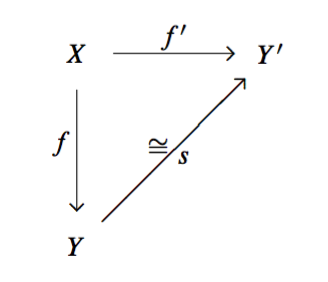
\includegraphics[width=5cm]{./Img/similar.png}
        \caption{Similar two surjective maps}
        \end{center}
    \end{figure}
    \begin{proposition}
        Two surjective maps $f: X \rightarrow Y$ and $f': X \rightarrow Y'$ determine the same equivalence relation X if and only if f and $f'$ are similar.
    \end{proposition}
    \begin{definition}[Canonical projection]
        The set of left cosets of H in G is denoted G/H . The surjective map $\pi : G \rightarrow G/H$ defined by $\pi(a) = aH$ is called the \textbf{canonical projection} or \textbf{quotient map} of G onto G/H.
    \end{definition}

    \begin{proposition}
    The fibers of the canonical projection $\pi : G \rightarrow G/H$ are the left cosets of H in G. The equivalence relation $\sim_{\pi}$ on G determined by $\pi$ is the equivalence relation $\sim_H$.
    \end{proposition}
    \subsubsection{Conjugacy}
        \begin{definition}[Conjugate]
            Let a and b be elements of a group G. We say that b is conjugate to a if there is a $g \in G$ such that $b = gag^{-1}$.
        \end{definition}
        
        \begin{definition}[Conjugacy classes]
            The equivalence classes for conjugacy are called conjugacy classes.
        \end{definition}
    \subsection{Quotient Groups and Homomorphism Theorems}

    \begin{theorem}
        Let N be a normal subgroup of a group G. The set of cosets G/N has a unique product that makes G=N a group and that makes the quotient map $\pi : G  \rightarrow G/N$ a group homomorphism, $ker(\pi) = N$.
    \end{theorem}
    
    \begin{proposition}
    	Let $a, b,c \in G$ and $N \unlhd G$, we have:
    		\begin{itemize}
    			\item Closure: $aNbN = abN$
    			\item Associativity: $aN(bNcN) = aNbNcN$
    			\item Identity: $aN(N) = (N)aN = aN$
    			\item Inverse: $(a^{-1}N)(aN) = (aN)(a^{-1}N) = N$
    		\end{itemize}
    \end{proposition}

    \subsubsection{Homomorphism Theorems}
    
        \begin{theorem}[Homomorphism theorem]
        Let $\varphi: G \rightarrow\bar{G}$ be a surjective homomorphism with kernel N. Let $\pi: G \rightarrow G/N$ be the quotient homomorphism. There is a group isomorphism $\tilde{\varphi}: G/N \rightarrow \bar{G}$ satisfying $\tilde{\varphi} \circ \pi = \varphi$.
        \[G / Ker(\phi) \cong \phi(G)\]
        \end{theorem}
        \begin{theorem}[Correspondence Theorem]
        Let $\varphi: G \rightarrow \bar{G}$ be a homomorphism of $G$ and $\bar{G}$, and let N denote the kernel of $\varphi$.
        \begin{enumerate}
            \item The map $\bar{B} \mapsto \varphi^{-1}(\bar{B})$ is a bijection between subgroups of $\bar{G}$ and subgroups of G containing N.
            \item Under this bijection, normal subgroups of $\bar{G}$ correspond to normal subgroups of G.
        \end{enumerate}

        \end{theorem}
        \begin{proposition}[Third Isomorphism Theorem]
            Let $\varphi: G \rightarrow \bar{G}$ be a surjective homomorphism with kernel N. Let $\bar{K}$ be a normal subgroup of $\bar{G}$ and let $K = \varphi^{-1}(\bar{K})$. Then $G=K \cong \bar{G}=\bar{K}$. Equivalently, $G/K \cong(G/N)(K/N)$.
        \end{proposition}

        \begin{theorem}[Factorization Theorem]
            Let $\varphi: G \rightarrow \bar{G}$ be a surjective homomorphism of groups with kernel K. Let $N\subseteq K$ be a subgroup that is normal in G, and let $\pi: G \rightarrow G/N$ denote the quotient map. Then there is a surjective homomorphism $\tilde{\varphi}: G/N \rightarrow G$ such that $\tilde{\varphi} \circ \pi = \varphi$. The kernel of $\tilde{\varphi}$ is $K/N \subseteq G/N$.
        \end{theorem}
        \begin{corollary}
            Let $N \subseteq K \subseteq G$ be subgroups with both N and K normal in G. Then $xN \mapsto xK$ defines a homomorphism of $G/N$ onto $G/K$ with kernel $K/N$.
        \end{corollary}
        \begin{theorem}[Second Isomorphism Theorem(Diamond)]
            Let $\varphi: G \rightarrow \bar{G}$ be a surjective homomorphism with kernel N. Let A be a subgroup of G. Then
            \begin{enumerate}
                \item $\varphi^{-1}(\varphi(A)) = AN = \{an : a \in A\ \mathrm{and}\ n \in N\}$,
                \item AN is a subgroup of G containing N.
                \item $AN/N \cong \varphi(A) \cong A/(A \cap N)$.
            \end{enumerate}
        \end{theorem}
        \begin{figure}[H]
        \begin{center}
        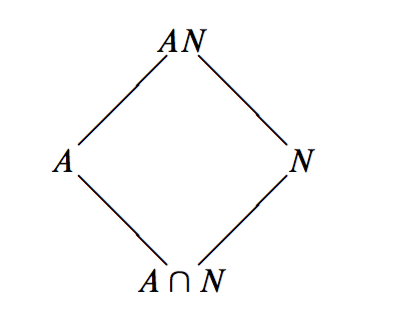
\includegraphics[width=7cm]{./Img/diamond.png}
        \caption{Diamond Isomorphism Theorem}
        \end{center}
        \end{figure}
        
        \begin{corollary}
        	\[gcd(m, n)\mathbb{Z}/n\mathbb{Z} \cong m\mathbb{Z} / lcm(m, n)\mathbb{Z}\]
        \end{corollary}
        
      \begin{proposition}[Fourth Isomorphism Theorem(Lattice)]
      	Let $\varphi: G \rightarrow H$ be a surjective group homomorphism, $N \ \mathrm{ker}(\varphi)$
      	we have 
      	\begin{enumerate}
      		\item There is a bijection \[\{subgroups\ of\ G\ containing\ N\} \leftrightarrow \{subgroups\ of\ H \cong G/N\}\]
      		\item Normalness is preserved by this bijection
      	\end{enumerate}
      \end{proposition}
      
      \begin{proposition}
      	If $H \subseteq G$ and $|G| / |H| = 2$, $H \unlhd G$.
      \end{proposition}  
        
        
    \section{Products of Groups}
    \subsection{Direct Products}
    \begin{definition}[Direct Product]
        $A \times B$, with this group structure, is called the direct product of A and B.
    \end{definition}
    \begin{proposition}
        Properties:
            \begin{enumerate}
                \item Suppose M and N are normal subgroups of G, and $M \cap N = \{e\}$. Then for all $m \in M$ and $n \in N$, $mn = nm$.
                \item $MN = \{mn: m \in M, n \in N\}$ is a subgroup and $(m, n) \mapsto mn$ is an isomorphism of $M \times N$ onto MN.
                \item If $MN = G$, then $G \cong M \times N$.
            \end{enumerate}
    \end{proposition}
    \begin{definition}[Direct Product]
        $A_1 \times A_2 \times \cdots \times A_n$, with the coordinate-by-coordinate multiplication, is called the \textbf{direct product} of $A_1, A_2, ..., A_n$.
    \end{definition}

    \begin{proposition}
        Suppose $N_1, N_2, ..., N_r$ are normal subgroups of a group G such that for all i,
            \[N_i \cap (N_1 ... N_{i-1}N_{i+1}...N_r) = {e}.\]
        Then $N_1N_2...N_r$ is a subgroup of G and $(n_1, n_2, ..., n_r) \mapsto n_1n_2...n_r$ is a subgroup of $P = N_1 \times N_2 \times \cdots \times N_n$ onto $N_1N_2...N_r$. In particular, if $N_1N_2...N_r = G$, then $G \cong N_1 \times N_2 \times \cdots \times N_n$.
    \end{proposition}

    \begin{corollary}
        Let $N_1, N_2, ... , N_r$ be normal subgroups of a group G such that $N_1N_2\cdots N_r = G$. Then G is the \textbf{internal direct product} of $N_1, N_2, ... , N_r$ if and only if whenever $x_i \in N_i$ for $1 \leq i \leq r$ and $x_1x_2\cdots x_r = e$, then $x_1 = x_2 = \cdots = x_r = e$.
    \end{corollary}

    \begin{definition}[Direct Sum]
        The \textbf{direct sum} of several rings $R_1, R_2, ..., R_n$ is the Cartesian product $R_1 \times R_2 \times \cdots \times R_n$, endowed with the coordinate-by-coordinate operations
            \[(r_1, r_2, ..., r_n) + (r'_1, r'_2, ..., r'_s) = (r_1 + r'_1, r_2 + r'_2, ..., r_n + r'_n)\]
            and
            \[(r_1, r_2, ..., r_n)(r'_1, r'_2, ..., r'_s) = (r_1r'_1, r_2r'_2, ..., r_nr'_n).\]
        The direct sum of $R_1, R_2, ..., R_n$ is denoted $R_1 \oplus R_2 \oplus ... \oplus R_n$.
    \end{definition}
    \begin{proposition}
    	If $m, n \in \mathbb{N}$, $g.c.d(m,n) = 1$, then \[\mathbb{Z}_{mn} \cong \mathbb{Z}_m \times \mathbb{Z}_n.\]
    \end{proposition}
    \begin{proposition}[Chinese Remainder Theorem]
        Let $n  \geq 2$ and let $a_1, ..., a_n$ be pairwise relatively prime natural numbers. Write a $a = a_1a_2...a_n$. Then
            \[ [x]_a \mapsto ([x]_{a_1}, [x]_{a_2}, ..., [x]_{a_n})\]
        defines a ring isomorphism
            \[\mathbb{Z}_a\cong \mathbb{Z}_{a_1} \oplus \mathbb{Z}_{a_2} \oplus ... \oplus \mathbb{Z}_{a_n}.\]
    \end{proposition}
    \begin{proposition}[Chinese Remainder Theorem]
        Let $n \geq 2$ and let $a_1 , a_2 , ... ,a_n$ be pairwise relatively prime natural numbers. Write $a = a_1a_2 \cdots a_n$. For any integers $x_1,x_2, ..., x_s$, there exists an integer x such that
        \[x \equiv x_i \mod a_i, for\ 1 \leq i \leq n.\]
        Moreover, x is unique up to congruence mod a.
    \end{proposition}
    \subsection{Semidirect Products}
    \begin{definition}[Semidirect Product]
        If we have groups N and A, and we have a homomorphism $\alpha : a \mapsto \alpha_a$ from A into the automorphism group Aut(N) of N, we can build from these data a new group $N \rtimes_{\alpha} A$, called the \textbf{semidirect product} of A and N . The semidirect product $N \rtimes_{\alpha} A$ has the following features: It contains (isomorphic copies of) A and N as subgroups, with N normal; the intersection of these subgroups is the identity, and the product of these subgroups is $N \rtimes_{\alpha} A$; and we have the commutation relation $an = \alpha_a(n)a$ for $a \in A$ and $n \in N$.
    \end{definition}

    \begin{proposition}
        Let N and A be groups, and $\alpha: A \rightarrow Aut(N)$ a homomorphism of A into the automorphism group of N. The Cartesian product $N \times A$ is a group under the multiplication $(n, a)(n', a') = (n\alpha_a(n'), aa')$. This group is denoted $N \rtimes_{\alpha} A$. This group is denoted $N \rtimes_{\alpha} A$. $\tilde{N} = \{(n, e):n \in N\}$ and $\tilde{A} = \{(e, a): a \in A\}$ are subgroups of $N \rtimes_{\alpha} A$, with $\tilde{N} \cong N$ and $\tilde{A} \cong A$, and $\tilde{N}$ is normal in $N \rtimes_{\alpha} A$. We have $(e, a)(n, e) = (\alpha_a(n), e) = (\alpha_a(n), a)$ for all $n \in N$ and $a \in A$.
    \end{proposition}
    \begin{corollary}
        Suppose G is a group, N and A are subgroups with N normal, $G = NA = AN$, and $A\cap N = {e}$. Then there is a homomorphism $\alpha: A \rightarrow Aut(N)$ such that G is isomorphic to the semidirect product $N \rtimes_{\alpha} A$.
    \end{corollary}
    \subsection{Vector Spaces}
        \begin{definition}[Vector Space]
            A \textbf{vector space} V over a field K is an abelian group with a product $K \times V \rightarrow V$, $(\alpha, v) \mapsto \alpha v$ satisfying the following conditions:
                \begin{enumerate}
                    \item $\forall v \in V, 1v = v.$
                    \item $\forall \alpha, \beta \in K, v \in V, (\alpha\beta)v = \alpha(\beta v).$
                    \item $\forall \alpha \in K, v,w \in V, \alpha(v + w) = \alpha v + \alpha w.$
                    \item $\forall \alpha , \beta \in K, v \in V, (\alpha + \beta)v = \alpha v + \beta v.$
                \end{enumerate}
        \end{definition}
        \begin{lemma}
            Let V be a vector space over the field K, then $\forall \alpha \in K, v \in V$,
            \begin{enumerate}
                \item $0v = \alpha 0 = 0.$
                \item $\alpha (-v) = -(\alpha v) = (-\alpha)v.$
                \item $(-1)v = -v.$
                \item $If \alpha \neq 0$ and $v \neq 0$, then $\alpha v \neq 0.$
            \end{enumerate}
        \end{lemma}

        \begin{definition}[Linear Transformation]
            Let V and W be vector spaces over K. A map $T: V \rightarrow W$ is called a \textbf{linear transformation} or \textbf{linear map} if $\forall x,y \in V, T(x + y) = T(x) + T(y)$ and $\forall \alpha \in K and x \in V, T(\alpha x) = \alpha T(x)$. An endomorphism of a vector space V is a linear transformation $T: V \rightarrow V$.
        \end{definition}
        \begin{definition}[Subspace]
            A subspace of a vector space V is a (nonempty) subset that is a vector space with the operations inherited from V.
        \end{definition}
        \begin{proposition}
            For a nonempty subset of a vector space to be a subspace, it suffices that the subset be closed under addition and under scalar multiplication.
        \end{proposition}

        \begin{proposition}
            Let $T : V \rightarrow W$ be a linear map between vector spaces. Then the range of T is a subspace of W and the kernel of T is a subspace of V.
        \end{proposition}
        \subsubsection{Quotients and homomorphism theorems}
            \begin{theorem}[Homomorphism theorem for vector spaces]
                If W is subspace of a vector space V over K, then $V/W$ has the structure of a vector space, and the quotient map $\pi: v \mapsto v + W$ is a surjective linear map from V to $V/W$ with kernel equal to W.
            \end{theorem}

            \begin{proposition}[Correspondence theorem for vector spaces]
                Let $T: V \rightarrow \bar{V}$ be a surjective linear map, with kernel N. Then $\bar{M} \mapsto T^{-1}(\bar{M})$ is a bijection between subspaces of V and subspaces of $\bar{V}$ containing N.
            \end{proposition}

            \begin{proposition}
                Let $T: V \rightarrow \bar{V}$ be a surjective linear transformation with kernel N. Let $\bar{M}$ be a subspace of V and let $M = T^{-1}(bar{M})$. Then $x + M \mapsto T(x) +  \bar{M}$ defines a linear isomorphism of $V/M$ to $\bar{V}/\bar{M}$. Equivalently,
                    \[(V/N)(M/N) \cong V/M,\]
                as vector spaces.
            \end{proposition}

            \begin{proposition}[Factorization Theorem for Vector Spaces]
                Let V and $\bar{V}$ be vector spaces over a field K, and let $T: V \rightarrow \bar{V}$ be a surjective linear map with kernel M. Let $N \subseteq M$ be a vector subspace and let $\pi: V \rightarrow V/N$ denote the quotient map. Then there is a surjective homomorphism $\tilde{T}: V/N \rightarrow \bar{V}$ such that $\tilde{T} \circ \pi = T$. The kernel is $M/N \subseteq V/N$.
            \end{proposition}
            \begin{proposition}[Diamond Isomorphism Theory for Vector Spaces]
                Let A and N be subgroups of a vector space V. Let $\pi$ denote the quotient map $\pi: V \rightarrow V/N$. Then $\pi^{-1}(\pi(A)) = A + N$ is a subspace of V containing both A and N. Furthermore, $(A + N)/N \cong \pi(A) \cong A/(A \cap N)$.
            \end{proposition}

                    
                    
                    \subsection{Finitely Generated Abelian Groups}
                    \begin{definition}
                    	$S$ generates $G$ if $\mathbb{Z}S = G$.
                    \end{definition}
                    
                    \begin{definition}
                    	$G$ is \textbf{finitely generated} if there is a finite set $S \subseteq G$ so that $\mathbb{Z}S = G$.
                    \end{definition}
                    
                    \begin{definition}
                    	G is \textbf{finitely generated} if there is  $S \subseteq G$ that is finite and $\mathbb{Z}S = G$.
                    \end{definition}
                    
                    \begin{definition}
                    	If $S$ generates $G$ and is linearly independent, say $S$ is a \textbf{basis} of G.
                    \end{definition}
                    
                    \begin{definition}
                    	If $G$ has a basis, then call $G$ a free group.
                    \end{definition}
                    
                    \begin{proposition}
                    	Let G be an abelian group and let $x_1, \cdots , x_n$ be distinct nonzero elements of G, the set $B =\{x_1,\cdots ,x_n\} $ is a basis of $G$ if and only if $G \equiv \mathbb{Z}^n$.
                    \end{proposition}
                    
                    \begin{theorem}[Fundamental Theorem of Finitely Generated Abelian Groups]
                    	Let G be a finitely generated abelian group.
                    	\begin{enumerate}
                    		\item G is a direct product of cyclic groups,
                    		\[G \cong \mathbb{Z}_{a_1} \times \mathbb{Z}_{a_2} \times \cdots \times \mathbb{Z}_{a_S} \times \mathbb{Z}^k\]
                    	\end{enumerate}
                    \end{theorem}
            
					\begin{definition}
						Let $g \in G$, if there is $n \neq 0$ so that $ng = 0$, call $g$ a torsion element. 
					\end{definition}
					
					\begin{proposition}
						If $x + G_{tor} \in G / G_{tor}$, $G / G_{tor} = 0 + G_{tor}$
					\end{proposition}
	\section{Group Actions}
		\begin{definition}
			An action of a group $G$ on a set $X$, a group action is a map $G \times X \rightarrow X$, denote as $gx_1 = x_2$
				\begin{itemize}
					\item $(g_1g_2)\cdot x = g_1(g_2x)$
					\item $ex = x$
					\item $x(g_1g_2) = xg_1g_2$
					\item $xe = x$
				\end{itemize}
		\end{definition}
		\begin{definition}
			Let $G$ act on $X, x \in X$. The orbit of $x$ denoted $G \cdot x$ or $\mathcal{O}(x)$, is the set $\{g \cdot x | g \in G\}$.
		\end{definition}
		
		\begin{definition}
			$x \sim y \Leftrightarrow y = g\cdot x$ for some $g \in G$. $\sim$ is an equivalent relation.
		\end{definition}
		\paragraph{Eg 1.} $G$ acts on itself by left multiplication: $g \cdot a = ga$.
		
		\begin{definition}
			If $G \curvearrowright X$ is one orbit, the action is called transitive.
		\end{definition}
		
		\paragraph{Eg 2.} $G \curvearrowright G / H$ by left transilation $g \cdot (aH) = (ga)H$
		
		\paragraph{Eg 3.1.} $H \subseteq G$. $H$ acts on $G$ by right multiplication $g \cdot h = gh$ with orbits are left cosets.
		
		\paragraph{Eg 3.2.}$H$ can also act on the left, with orbits to be the right cosets.
		
		\paragraph{Eg 4.} G acts on itself by conjugation. $g /cdot a = gag^{-1}$ with orbits to be conjugacy classes.
		\begin{definition}[Stablizer]
			Let $G$ acts on $X$. The stablizer $Stab_G(X) = \{g \in G| gx = x\}$.
		\end{definition}
		\begin{proposition}
			$Stab_G(X) \subseteq G$
		\end{proposition}
		
		\begin{theorem}
			Let $G$ acts on $X$,  $x \in X$. There is a natural bijection $\phi: G / Stab_G(x) \rightarrow G \cdot X$
		\end{theorem}
		
		\begin{theorem}[Orbit-Stablizer Theorem]
			\[|\mathcal{O}(x)| = \frac{|G|}{|Stab(x)|}\]
		\end{theorem}
		
		\begin{definition}[Normalizer]
			Consider the action of a group G on its subgroups by conjugation. The stabilizer of a subgroup H is called the normalizer of H in G and denoted $N_G(H)$.
		\end{definition}
		
		\begin{definition}[Centralizer]
			Consider the action of a group G on its subgroups by conjugation. The stabilizer of an element $g \in G$ is called the centralizer of $g$ in $G$ and denoted $Cent_G(H)$.
		\end{definition}
		
		\subsection{Group Actions and counting}
		
		\begin{definition}
			For $g \in G$, let $Fix(g) = \{x \in X : gx = xg\}$
		\end{definition}
		
		\begin{proposition}
			Let a finite group $G$ act on a finite set $X$. Then the number of orbits of the action is
			\[\mathrm{\#\ of\ orbits} = \frac{1}{|G|} \sum_{g \in G}|\mathrm{Fix}(g)|\]
		\end{proposition}
		
		\subsection{Group Automorphisms}
			\begin{definition}
				If $G$ is a group, then automorphism $\mathrm{Aut}(G) = \{\varphi: G \rightarrow G | \varphi\ \mathrm{is\ isomorphism}\}$. 
			\end{definition}
			
			\begin{definition}
				$\mathrm{Int}(G) = \{c_g | g\in G\}$ for each $g \in G, c_g: G \rightarrow G$ and $c_g(x) = gxg^{-1}$.
			\end{definition}
			
			\begin{proposition}
				$\mathrm{Int(G)} \subseteq \mathrm{Aut(G)}$
			\end{proposition}
			
			\begin{proposition}
				If $G$ is abelian, then $\mathrm{Int}(G) = \{1\}$
			\end{proposition}
			
			\begin{proposition}
				$\mathrm{Int}(G) \cong G / Z(G)$
			\end{proposition}
			
			\begin{proposition}
				$\mathrm{Int}(G) \unlhd \mathrm{Aut}(G)$
			\end{proposition}
		
			\begin{proposition}
				$\mathrm{Aut}(\mathbb{Z}) \cong \mathbb{Z}_2$. If $p$ is a prime, $\mathrm{Aut}(\mathbb{Z}_p) = \mathbb{Z}_{p - 1}$
			\end{proposition}
		
		\subsection{Sylow Theorem}
		
			\begin{proposition}
				Suppose $p$ is a prime, $|G| = p^n$. Then $Z(G)$ contains nonidentity elements.
			\end{proposition}
		
			\begin{corollary}
				Suppose $p$ is prime and $|G| = p^2$, then $G \cong \mathbb{Z}_{p^2}$ or $G \cong \mathbb{Z}_p \times \mathbb{Z}_p$.
			\end{corollary}
			\begin{definition}
				$|G| = p^n$, then there is a normal subgroup $N \unlhd G, \{e\} \subsetneq N \subsetneq G$, such that all subgroups of $N$ are normal.
			\end{definition}
			
			\begin{corollary}
				$|G| = p^n$, $p$ is prime, then there exists subgroups $\{e\} = G_0 \subseteq G_1 \subseteq \cdots \subseteq G_n = G$ such that $|G_k| = p^k$ and each $G_k \unlhd G.$
			\end{corollary}
			
			\begin{theorem}[Cauchy's Theorem]
				Suppose $p$ is prime and $p | |G|$, then $G$ has an element of order $p$.
			\end{theorem}
			
			\begin{definition}
				$G$ is a finite group, $p$ is prime. If $p^n$ is the largest power of $p$ dividing $|G|$ then a subgroup of size $p^n$ is a \textbf{p-Sylow subgroup} of $G$.
			\end{definition}
		
		
			\begin{theorem}[1st Sylow Theorem]
				If $p^n | |G|$ then $G$ has a subgroup of size $p^n$.
			\end{theorem}
		
			\begin{theorem}[2nd Sylow Theorem]
				Let $P, Q$ be $2$ p-Sylow subgroups. Then $P$ and $Q$ are conjugate subgroups. ($g \in G, gPg^{-1} = Q$)
			\end{theorem}
			
			\begin{corollary}
				There is exactly $1$ p-Sylow subgroup if and only if the subgroup is normal.
			\end{corollary}
			
			\begin{theorem}[3rd Sylow Theorem]
				If $p^n$ is the order of a p-Sylow subgroup of $G$, the number of p-Sylow subgroups of $G$ satisfies
					\begin{itemize}
						\item $\# \equiv 1 \mod p$
						\item $\#$ divides $\frac{|G|}{p^n}$
					\end{itemize}
			\end{theorem}
		
		
		\section{Ring}
		
		\subsection{Basics}
		
		\begin{definition}[Ring]
			A \textbf{ring} with two operations $+, \cdot$, if 
			\begin{enumerate}
				\item $R, +$ is an abelian group with identity:0 and inverses $-a$,
				\item $R, \cdot$ is closed and associative
				\item $R, +, \cdot$ is distributive.
			\end{enumerate}
		\end{definition}
		
		\subsection{Homomorphism and Ideal}
		\begin{definition}[Ring homomorphism]
			A \textbf{ring homomorphism} $\varphi: R \rightarrow S$ is a map which preserves addition and multiplication.
			
			Let $a, b \in R$, we have:
			\begin{enumerate}
				\item $\varphi(a + b) = \varphi(a) + \varphi(b)$
				\item $\varphi(ab) = \varphi(a)\varphi(b)$
			\end{enumerate}
			
			$\varphi$ is an \textbf{isomorphism} if it is also bijection.
		\end{definition}
		
		\begin{definition}
			An element of a ring with multiplicative inverse is called a \textbf{unit}.
		\end{definition}
		
		\begin{definition}
			A left(right) \textbf{ideal} of a ring $R$, is a subset $I \subseteq R$ that 
			\begin{enumerate}
				\item $I \subseteq R$
				\item If $r \in R$, $a \in I$, then $ra \in I(ar \in I)$
			\end{enumerate}
			\footnote{Check if $I \subseteq R$ is an ideal: \begin{enumerate}
				\item $I \neq \emptyset$
				\item If $a, b \in I$, $ar - b \in I$
			\end{enumerate}}
		\end{definition}
		
		\begin{proposition}
			If $\varphi: R \rightarrow S$ is a ring homomorphism, then $\mathrm{Ker}(\varphi)$ is a (left and right) ideal of $R$.
		\end{proposition}
		
		\begin{proposition}
			If an ideal contains a unit, then it contains the whole ring.
		\end{proposition}
		
		\begin{proposition}
			If a ring is a field, then its ideal is either $\{0\} $ or the whole ring.
		\end{proposition}
		
		\begin{proposition}
			\begin{itemize}
				\item If $\{I_{\alpha}\}$ is ideals of $R$, then $\bigcap I_{\alpha}$ is an ideal.
				\item If $I_1 \subseteq I_2 \subseteq \cdots$ are ideals of $R$, then $\bigcup I_i$ is an ideal.
			\end{itemize}
		\end{proposition}
		
		\subsubsection{Ideals generated by sets}
			\begin{definition}
				Let $S \subseteq R$ and $S \neq \emptyset$, then the \textbf{ideal generated by S} (S), the smallest ideal of $R$ containing $S$.
				
				If $S = \{a\}$, $(S) = (a)$ is called a \textbf{Principal ideal}.
			\end{definition}
		\subsection{Quotient Ring}
			\begin{proposition}
				Let $I$ is an ideal of $R$, $R/I = \{r + I | r \in R\}$ is a ring.
			\end{proposition}
			
			\begin{definition}
				Say $a$ is a zero-divisor, if $\exists b$ that $ab = 0$.
			\end{definition}
			
			
			\subsubsection{Four Isomorphism Theorem for Ring}
			\begin{theorem}[First]
			 If $\varphi: R \rightarrow S$ surjective ring hom with kernel $I$, then $R/I \cong S$.	
			\end{theorem}
			\paragraph{Ex.} $ev_0: \mathbb{Z}[x] \rightarrow \mathbb{Z} \Rightarrow \mathbb{Z}[x]/(x) = \mathbb{Z}$.
			
			\begin{theorem}[Second]
				If $I$ is an ideal of $R$ and $A$ is a subring, then $(A + I) / I \cong A / A \cap I$.
			\end{theorem}
			
			\begin{theorem}[Third]
				If $J \subseteq I$ are ideals of $R$, then $(R/J)/(I/J) \cong R/I$.
			\end{theorem}

			\begin{theorem}[Fourth]
				Let $I \subseteq R$ be an ideal, then there is one-to-one correspondence $\{ideals\ of\ R/I\} \leftrightarrow \{ideals\ of\ R\ containing\ I\}$ 
			\end{theorem}
			
			\begin{definition}
				An ideal $M$ of $R$ is \textbf{maximal} if whenever an ideal $M \subseteq I \subseteq R$ then $I = M$ or $I = R$.
			\end{definition}	
			
			\paragraph{Ex.} $2\mathbb{Z}$ is a maximal ideal of $\mathbb{Z}$.
			
			\begin{proposition}
				Let $R$ be commutative with multiplicative identity $1$. Then $M$ is a max ideal $\Leftrightarrow R / M$ is a field.
			\end{proposition}		
			
\end{document}
